We now evaluate the performance of PES in the task of finding the optimum of
synthetic black-box objective functions.  For this, we reproduce the within-model
comparison experiment described in \cite{HennigSchuler:2012}.  In this
experiment we optimize objective functions defined in the 2-dimensional unit domain
$\X = [0,1]^2$.  Each objective function is generated by first sampling 1024 function
values from the GP prior assumed by PES, using the same $\gamma^2$, $\ell_i$ and $\sigma^2$
as in the previous experiment.  The objective function is then given by the resulting
GP posterior mean.  We generated a total of 1000 objective functions by following
this procedure.  The left plot in Figure \ref{fig:resultsSyntheticFunctions}
shows an example function.  

In these experiments we compared the performance of PES with that of ES
\cite{HennigSchuler:2012} and expected improvement (EI) \cite{Jones:1998}, a
widely used acquisition function in the Bayesian optimization literature.  We
again assume that the optimal hyper-parameter values are known to all methods.
Predictive performance is then measured in terms of the immediate regret (IR)
$|f(\xrec_n) - f(\xopt)|$, where $\xopt$ is the known location of the global
maximum and $\xrec_n$ is the recommendation of each algorithm had we stopped at
step $n$---for all methods this is given by the maximizer of the posterior mean.
The right plot in Figure \ref{fig:resultsSyntheticFunctions} shows the decimal
logarithm of the median of the IR obtained by each method across the 1000
\emph{different} objective functions.  Confidence bands equal to one standard
deviation are obtained using the bootstrap method.  Note that while averaging
these results is also interesting, corresponding to the expected performance
averaged over the prior, here we report the median IR because
the empirical distribution of IR values is very heavy-tailed.  In this case, the
median is more representative of the exact location of the bulk of the data.
%Note also that were one to average these results it is important to average
%before transforming to logspace in order to not inadvertently suppress outliers.
These results indicate that the best method in this setting is PES, which
significantly outperforms ES and EI.  The plot also shows that in this case ES
is significantly better than EI.

\begin{figure}
\begin{center}

\includegraphics[width=0.7\linewidth]{figures/experimentSyntheticFunctions/figure.pdf}
\end{center}
\vspace{-1em}
\caption{\small Left, example of objective functions $f$. Right, median of the immediate
regret (IR) for the methods PES, ES and EI in the experiments with synthetic
objective functions.} \label{fig:resultsSyntheticFunctions}
\end{figure}

We perform another series of experiments in which we optimize well-known
synthetic benchmark functions including a mixture of cosines
\cite{Anderson:2000} and Branin-Hoo (both functions defined in $[0,1]^2$) as well as the
Hartmann-6 (defined in $[0,1]^6$) \cite{Lizotte:2008}.  In all instances, we fix the
measurement noise to $\sigma^2 = 10^{-3}$.  For both PES and EI we marginalize
the hyperparameters $\vpsi$ using the approach described in Section
\ref{sec:hyper-learning}.  ES, by contrast, cannot average its approximation of
(\ref{eq:originalObjective}) over the posterior on $\vpsi$.  Instead, ES works
by fixing $\vpsi$ to an estimate of its posterior mean (obtained using slice
sampling) \cite{Vanhatalo:2012}.  To evaluate the gains produced by the fully
Bayesian treatment of $\vpsi$ in PES, we also compare with a version of PES
(PES-NB) which performs the same non-Bayesian (NB) treatment of $\vpsi$ as ES.
In PES-NB we use a single fixed hyperparameter as in previous sections with
value given by the posterior mean of $\vpsi$.  All the methods are initialized
with three random measurements collected using latin hypercube sampling
\cite{Brochu:2009}.

The plots in Figure \ref{fig:resultsAnalyticRealWorldFunctions} show the median
IR obtained by each method on each function across 250 random initializations.
Overall, PES is better than PES-NB and ES. Furthermore, PES-NB is also
significantly better than ES in most of the cases.  These results show that the
fully Bayesian treatment of $\vpsi$ in PES is advantageous and that PES can
produce better approximations than ES.  Note that PES performs better than EI in
the Branin and cosines functions, while EI is significantly better on the
Hartmann problem. This appears to be due to the fact that entropy-based
strategies explore more aggressively which in higher-dimensional spaces takes
more iterations. The Hartmann problem, however, is a relatively simple problem
and as a result the comparatively more greedy behavior of EI does not result in
significant adverse consequences. Note that the synthetic functions optimized in the
previous experiment were much more multimodal that the ones considered here.

\begin{figure}
\begin{center}
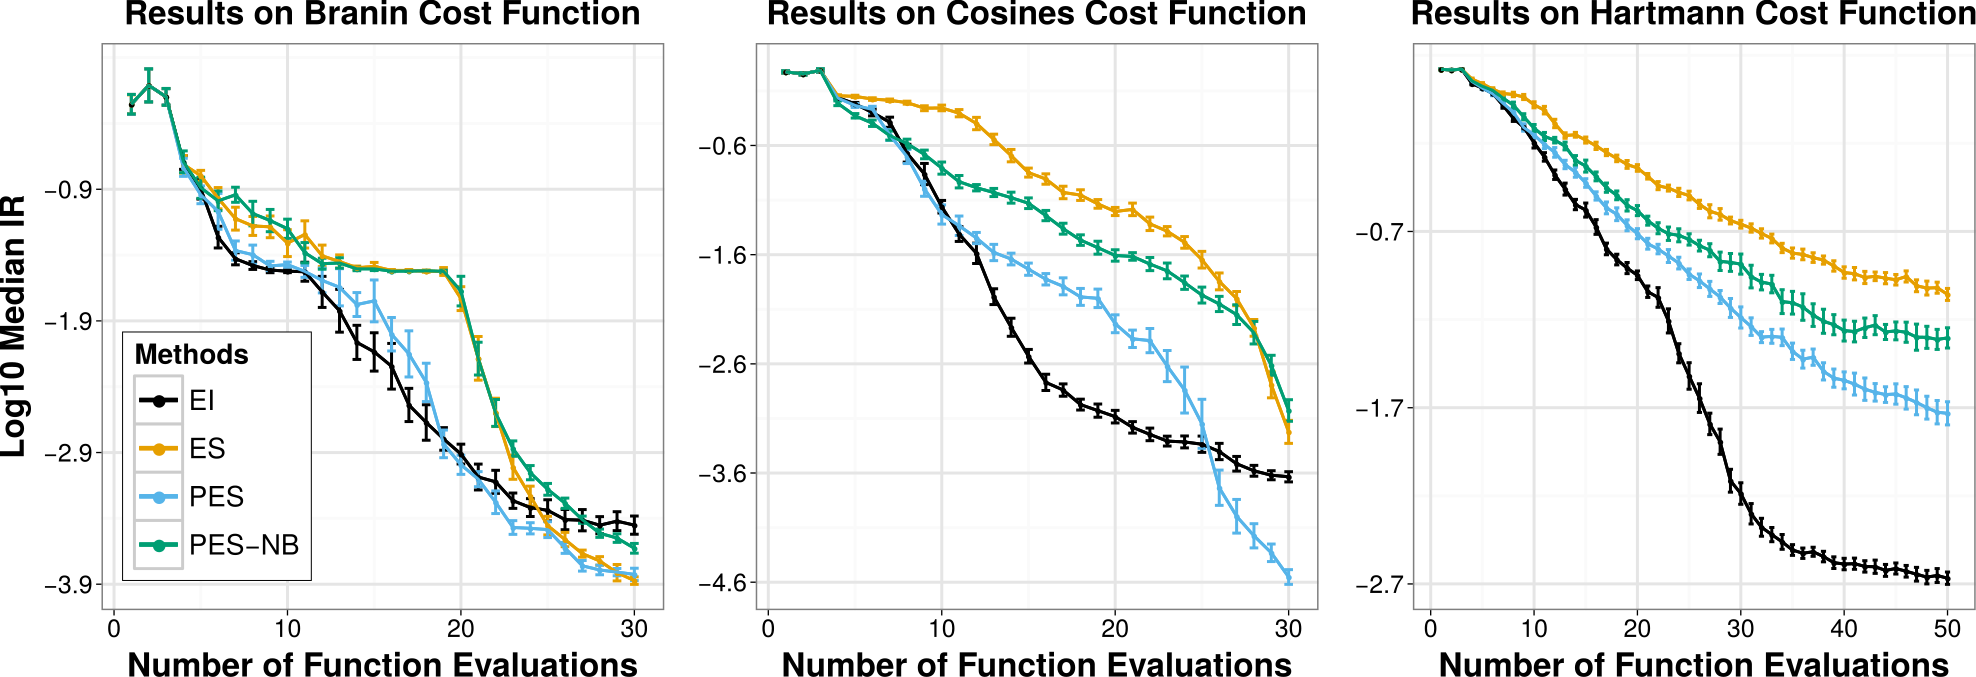
\includegraphics[width=0.85\linewidth]{figures/experimentAnalyticRealWorldFunctions/figure.pdf}
\end{center}
\vspace{-0.5em}
\caption{\small Median of the immediate regret (IR) for the methods EI, ES, PES and
PES-NB in the experiments with well-known synthetic benchmark functions.}
\label{fig:resultsAnalyticRealWorldFunctions}
\vspace{-1.0em}
\end{figure}
